\chapter[TorchIO: a software library for medical image processing]{TorchIO: a software library for medical image preprocessing and augmentation in deep learning}
% {TorchIO: a Python library for efficient loading, preprocessing, augmentation and patch-based sampling of medical images in deep learning}

\chaptermark{TorchIO: a library for medical image processing}
\label{chap:torchio}
\minitoc

\begin{center}
  \begin{minipage}[b]{0.9\linewidth}
    \small
    \textbf{Foreword\,}
    This chapter is an \textit{in extenso} reproduction of:
    \begin{itemize}
      \item \bibentry{perez-garcia_torchio_2021}
    \end{itemize}
  \end{minipage}
\end{center}

\definecolor{pytorch_orange}{HTML}{F84C36}

\section{Introduction}

\subsection{Motivation}

Approximately one third of epilepsies are drug-resistant.
If the \ac{EZ}, i.e., ``the area of cortex indispensable for the generation of clinical seizures'' \cite{rosenow_presurgical_2001}, can be localized, resective surgery to remove the \ac{EZ} may be curative.
As previously mentioned, only 40\% to 70\% of patients with refractory focal epilepsy are seizure-free after surgery \cite{jobst_resective_2015}.
This is, in part, due to limitations identifying the \ac{EZ} during the presurgical evaluation.
Retrospective studies relating presurgical clinical features and resected brain structures to surgical outcome provide useful insights to guide \ac{EZ} resection \cite{jobst_resective_2015}.
To quantify resected structures, first, the \ac{RC} must be segmented on the postoperative \ac{MRI}.
A preoperative image with a corresponding brain parcellation can then be registered to the postoperative \ac{MRI} to identify resected structures.

\Ac{RC} segmentation is also necessary in other applications.
For neuro-oncology, the gross tumor volume, which is the sum of the \ac{RC} and residual tumor volumes, is estimated for postoperative radiotherapy \cite{ermis_fully_2020}.

Despite recent efforts to segment \acp{RC} in the context of brain cancer \cite{meier_automatic_2017,ermis_fully_2020}, little research has been published in the context of epilepsy surgery.
Furthermore, previous work is limited by the lack of benchmark datasets, released code or trained models, and evaluation is restricted to single-institution datasets used for both training and testing.


\subsection{Related works}

After surgery, \acp{RC} fill with \ac{CSF}.
This causes an inherent uncertainty in delineating \acp{RC} adjacent to structures such as sulci, ventricles or edemas.
Nonlinear registration has been presented to segment the \ac{RC} for epilepsy \cite{chitphakdithai_non-rigid_2010} and brain tumor \cite{chen_deformable_2015} surgeries by detecting non-corresponding regions between pre- and postoperative images.
However, evaluation of these methods was restricted to a very small number of images.
Furthermore, in cases with intensity changes due to the resection (e.g., brain shift, atrophy, fluid filling), non-corresponding voxels may not correspond to the \ac{RC}.

Decision forests were presented for brain cavity segmentation after glioblastoma surgery, using four \ac{MRI} modalities \cite{meier_automatic_2017}.
These methods, which aggregate hand-crafted features extracted from all  modalities to train a classifier, can be sensitive to signal inhomogeneity and unable to distinguish regions with intensity patterns similar to \ac{CSF} from \acp{RC}.
Recently, a 2D \ac{CNN} was trained to segment the \ac{RC} on \ac{MRI} slices in 30 glioblastoma patients \cite{ermis_fully_2020}.
They obtained a `median (interquartile range)' \ac{DSC} of 84 (10) compared to ground-truth labels by averaging predictions across anatomical axes to compute the 3D segmentation.
While these approaches require four modalities to segment the \ac{RC}, some of the modalities are often unavailable in clinical settings \cite{dorent_learning_2021}.
Furthermore, code and datasets are not publicly available, hindering a fair comparison across methods.
Applying these techniques requires curating a dataset with manually obtained annotations to train the models, which is expensive.

Unsupervised learning methods can leverage large, unlabeled medical image datasets during training.
In self-supervised learning, training instances are generated automatically from unlabeled data and used to train a model to perform a pretext task. %such as inpainting or image restoration.
The model can be fine-tuned on a smaller labeled dataset to perform a downstream task \cite{chen_self-supervised_2019}.
The pretext and downstream tasks may be the same.
For example, a \ac{CNN} was trained to reconstruct a skull bone flap by simulating craniectomies on CT scans \cite{matzkin_self-supervised_2020}.
Lesions simulated in chest CT of healthy subjects were used to train models for nodule detection, improving accuracy compared to training on a smaller dataset of real lesions \cite{pezeshk_seamless_2017}.

% Recovered from long version
Semi-supervised learning may be used when a large amount of unlabeled data is available.
A model trained on a labeled dataset (which may have been generated in a self-supervised setting) can generate pseudolabels for unlabeled data.
Uncertainty estimation may be used to select pseudolabeled instances with a low uncertainty for medical image segmentation tasks, improving model performance compared to using a random subset \cite{venturini_uncertainty_2020}.


\subsection{Contributions}

We present a self-supervised learning approach to train a 3D \ac{CNN} for brain \acp{RC} segmentation from \ac{T1w} \ac{MRI} without annotated data, by simulating resections during training.
We performed a comprehensive evaluation of our framework, assessing the effect of the resection simulation shape on performance and evaluating datasets from different institutions and pathologies.
We used uncertainty estimation as a selection criterion for pseudolabeled instances within our semi-supervised learning setting, which can be leveraged when postoperative \acp{MRI} without annotation are available, a typical scenario in clinical settings.

We ensure our work is reproducible by releasing the source code for resection simulation and \ac{CNN} training, the trained \ac{CNN}, and the evaluation dataset.
To the best of our knowledge, we introduce the first open annotated dataset of postoperative \ac{MRI} for epilepsy surgery.

\subsection{Motivation}

The nature of medical images makes it difficult to rely on a typical computer-vision pipeline for neural network training.
In \cref{sec:challenges}, we describe challenges related to medical images that need to be overcome when designing deep learning workflows.
In \cref{sec:frameworks}, we justify the choice of PyTorch as the main deep learning framework dependency of TorchIO.

\subsubsection{Challenges in medical image processing for deep learning}
\label{sec:challenges}


In practice, multiple challenges must be addressed when developing deep learning algorithms for medical images:
1) handling metadata related to physical position and size,
2) lack of large labeled datasets,
3) high computational costs due to data multidimensionality and
4) lack of consensus for best normalization practices.
These challenges are very common in medical imaging and require certain features that may not be implemented in more general-purpose image processing frameworks such as Albumentations~\cite{buslaev_albumentations_2020} or TorchVision~\cite{paszke_pytorch_2019}.


\paragraph{Metadata}
\label{sec:metadata}

In computer vision, picture elements, or \textit{pixels}, which are assumed to be square, have a spatial relationship that comprises proximity and depth according to both the arrangement of objects in the scene and camera placement.
In comparison, medical images are reconstructed such that the location of volume elements, or cuboid-shaped \textit{voxels}, encodes a meaningful 3D spatial relationship.
In simple terms, for 2D natural images, pixel vicinity does not necessarily indicate spatial correspondence, while for medical images spatial correspondence between nearby voxels can often be assumed.

Metadata, which encodes the physical size, spacing, and orientation of voxels, determines spatial relationships between voxels~\cite{larobina_medical_2014}.
This information can provide meaningful context when performing medical image processing, and is often implicitly or explicitly used in medical imaging software.
Furthermore, metadata is often used to determine correspondence between images as well as voxels within an image.
For example, registration algorithms for medical images typically work with physical coordinates rather than voxel indices.

\cref{fig:metadata} shows the superposition of an \ac{MRI} and a corresponding brain parcellation~\cite{cardoso_geodesic_2015} with the same size ($181 \times 181$) but different origin, spacing and orientation.
A naïve user would assume that, given that the superimposition looks correct and both images have the same size, they are ready for training.
However, the visualization is correct only because 3D Slicer~\cite{fedorov_3d_2012}, the software used for visualization, is aware of the spatial metadata of the images.
As \acp{CNN} generally do not take spatial metadata into account, training using these images without preprocessing would lead to poor results.


\begin{figure}
  \centering

  \begin{subfigure}{0.24\textwidth}
    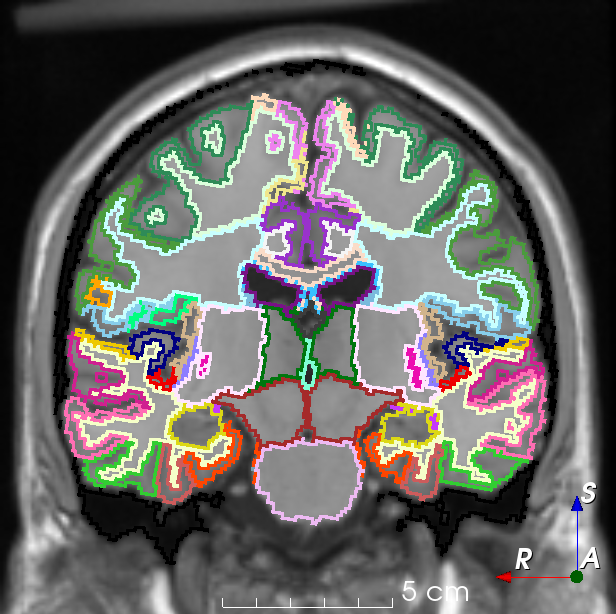
\includegraphics[width=\linewidth]{metadata_ok}
    \caption{}
    \label{fig:meta_ok}
  \end{subfigure}
  \hfill
  \begin{subfigure}{0.24\textwidth}
    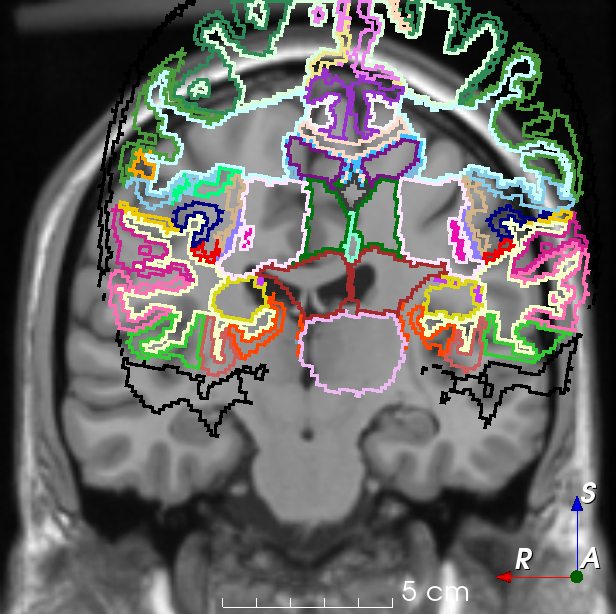
\includegraphics[width=\linewidth]{metadata_origin}
    \caption{}
    \label{fig:meta_origin}
  \end{subfigure}
  \hfill
  \begin{subfigure}{0.24\textwidth}
    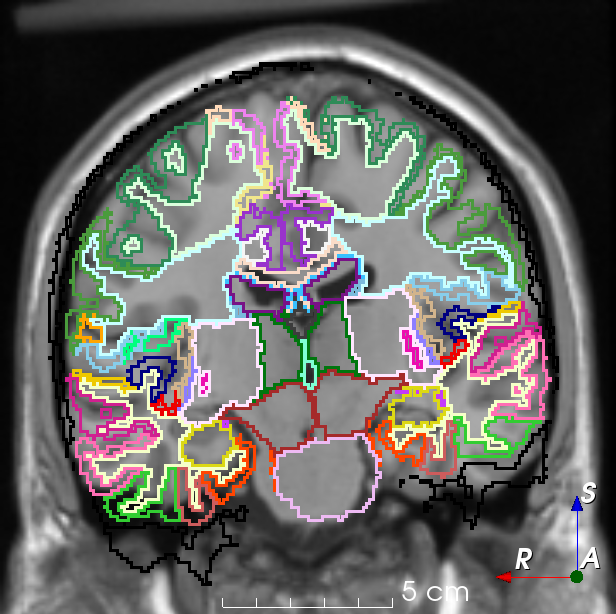
\includegraphics[width=\linewidth]{metadata_orientation}
    \caption{}
    \label{fig:meta_orientation}
  \end{subfigure}
  \hfill
  \begin{subfigure}{0.24\textwidth}
    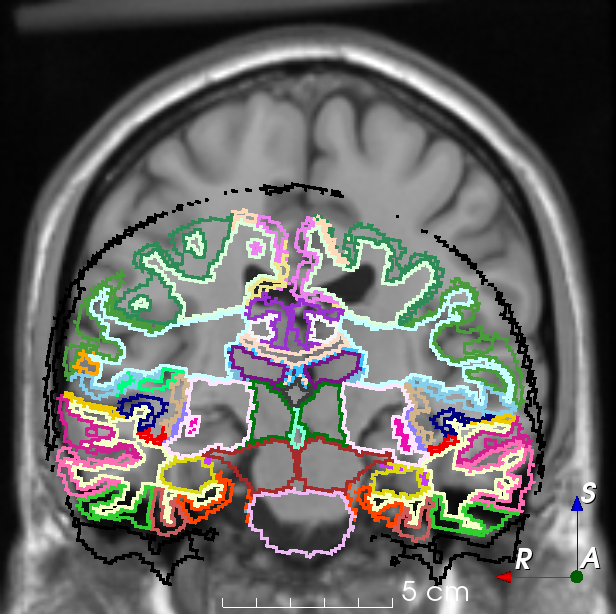
\includegraphics[width=\linewidth]{metadata_spacing}
    \caption{}
    \label{fig:meta_spacing}
  \end{subfigure}

  \caption[Importance of spatial metadata in medical imaging processing]{
    Demonstration of the importance of spatial metadata in medical image processing.
    The size of both the \ac{MRI} and the segmentation is $181 \times 181$.
    When spatial metadata is taken into account (\subref{fig:meta_ok}), images are correctly superimposed (only the borders of each region are shown for clarity purposes).
    Images are incorrectly superimposed if (\subref{fig:meta_origin}) origin, (\subref{fig:meta_orientation}) orientation or (\subref{fig:meta_spacing}) spacing are ignored.
  }
  \label{fig:metadata}
\end{figure}



Medical images are typically stored in specialized formats such as \ac{DICOM} or \ac{NIfTI}~\cite{larobina_medical_2014}, and commonly read and processed by medical imaging frameworks
such as SimpleITK~\cite{lowekamp_design_2013} or NiBabel~\cite{brett_nipynibabel_2020}.


\paragraph{Limited training data}

Deep learning methods typically require large amounts of annotated data, which are often scarce in clinical scenarios due to concerns over patient privacy, the financial and time burden associated with collecting data as part of a clinical trial, and the need for annotations from highly-trained and experienced raters.
Data augmentation techniques can be used to increase the size of the training dataset artificially by applying different transformations to each training instance while preserving the relationship to annotations.

Data augmentation performed in computer vision typically aims to simulate variations in camera properties, \ac{FOV}, or perspective.
Traditional data augmentation operations applied in computer vision include geometrical transforms such as random rotation or zoom, color-space transforms such as random channel swapping or kernel filtering such as random Gaussian blurring.
Data augmentation is usually performed on the fly, i.e., every time an image is loaded from disk during training.

Several computer vision libraries supporting data augmentation have appeared recently, such as Albumentations~\cite{buslaev_albumentations_2020}, or \texttt{imgaug}~\cite{jung_imgaug_2020}.
PyTorch also includes some computer vision transforms, mostly implemented as Pillow wrappers~\cite{wiredfool_pillow_2016}.
However, none of these libraries support reading or transformations for 3D images.
Furthermore, medical images are almost always greyscale, therefore colour-space transforms are not applicable.
Additionally, cropping and scaling are more challenging to apply to medical images without affecting the spatial relationships of the data.
Metadata should usually be considered when applying these transformations to medical images.

In medical imaging, the purpose of data augmentation is designed to simulate anatomical variations and scanner artifacts.
Anatomical variation and sample position can be simulated using spatial transforms such as elastic deformation, lateral flipping, or affine transformations.
Some artifacts are unique to specific medical image modalities.
For example, ghosting artifacts will be present in \ac{MRI} if the patient moves during acquisition, and metallic implants often produce streak artifacts in \ac{CT}.
Simulation of these artifacts can be useful when performing augmentation on medical images.


\paragraph{Computational costs}
\label{sec:computation}
The number of pixels in 2D images used in deep learning is rarely larger than one million.
For example, the input size of several popular image classification models is $224 \times 224 \times 3 = \num{150528}$ pixels (\SI{588}{\kibi\byte} if 32 bits per pixel are used).
In contrast, 3D medical images often contain hundreds of millions of voxels, and downsampling might not be acceptable when small details should be preserved.
For example, the size of a high-resolution lung \ac{CT}-scan used for quantifying chronic obstructive pulmonary disease damage in a research setting, with spacing $0.66 \times 0.66 \times 0.30$ mm, is $512 \times 512 \times 1069 = \num{280231936}$ voxels (\SI{1.04}{\gibi\byte} if 32 bits per voxel are used).


In computer vision applications, images used for training are grouped in batches whose size is often in the order of hundreds~\cite{krizhevsky_imagenet_2012} or even thousands~\cite{chen_simple_2020} of training instances, depending on the available \ac{GPU} memory.
In medical image applications, batches rarely contain more than one~\cite{cicek_3d_2016} or two~\cite{milletari_v-net_2016} training instances due to their larger memory footprint compared to natural images.
This reduces the utility of techniques such as batch normalization, which rely on batches being large enough to estimate dataset variance appropriately~\cite{ioffe_batch_2015}.
Moreover, large image size and small batches result in longer training time, hindering the experimental cycle that is necessary for hyperparameter optimisation.
In cases where \ac{GPU} memory is limited and the network architecture is large, it is possible that not even the entirety of a single volume can be processed during a training iteration.
To overcome this challenge, it is common in medical imaging to train using subsets of the image, or image \textit{patches}, randomly extracted from the volumes.

Networks can be trained with 2D slices extracted from 3D volumes, aggregating the inference results to generate a 3D volume~\cite{lucena_convolutional_2019}.
This can be seen as a specific case of patch-based training, where the size of the patches along a dimension is one.
Other methods extract volumetric patches for training, that are often cubes, if the voxel spacing is isotropic~\cite{li_compactness_2017}, or cuboids adapted to the anisotropic spacing of the training images~\cite{nikolov_deep_2018}.


\paragraph{Transfer learning and normalization}

One can pre-train a network on a large dataset of natural images such as ImageNet~\cite{deng_imagenet_2009}, which contains more than 14 million labeled images, and fine-tune on a custom, much smaller target dataset.
This is a typical use of transfer learning in computer vision~\cite{weiss_survey_2016}.
The literature has reported mixed results using transfer learning to apply models pretrained on natural images to medical images~\cite{cheplygina_cats_2019,raghu_transfusion_2019}.

In computer vision, best practice is to normalize each training instance before training, using statistics computed from the whole training dataset~\cite{krizhevsky_imagenet_2012}.
Preprocessing of medical images is often performed on a per-image basis, and best practice is to take into account the bimodal nature of medical images (i.e., that an image has a background and a foreground).

Medical image voxel intensity values can be encoded with different data types and intensity ranges, and the meaning of a specific value can vary between different modalities, sequence acquisitions, or scanners.
Therefore, intensity normalization methods for medical images often involve more complex parameterization of intensities than those used for natural images~\cite{nyul_standardizing_1999}.

\subsubsection{Deep learning frameworks}
\label{sec:frameworks}

There are currently two major generic deep learning frameworks: TensorFlow \cite{abadi_tensorflow_2016} and PyTorch \cite{paszke_pytorch_2019}, primarily maintained by Google and Facebook, respectively.
Although TensorFlow has traditionally been the primary choice for both research and industry, PyTorch has recently seen a substantial increase in popularity, especially among the research community \cite{he_state_2019}.

PyTorch is often preferred by the research community as it is \textit{pythonic}, i.e., its design, usage, and \ac{API} follow the conventions of plain Python. Moreover, the \ac{API} for tensor operations follows a similar paradigm to the one for NumPy multidimensional arrays, which is the primary array programming library for the Python language \cite{van_der_walt_numpy_2011}.
In contrast, for TensorFlow, researchers need to become familiar with new design elements such as sessions, placeholders, feed dictionaries, gradient tapes and static graphs.
In PyTorch, objects are standard Python classes and variables, and a dynamic graph makes debugging intuitive and familiar to anyone already using Python.
These differences have decreased with the recent release of TensorFlow 2, whose eager mode makes usage reminiscent of Python.

TorchIO was designed to be in the style of PyTorch and uses several of its tools to reduce the barrier to learning how to use TorchIO for those researchers already familiar with PyTorch.


